\section{Unsupervised}
This kind of learning is used when a dataset does not have any label $t$, so we need to cluster similar samples $x$ based of some other metrics.

\subsection{Gaussian Mixture Models }
One way is to assume the data is made of a mixture (sum) of gaussians , so we let the model maximize the probability of  \textit{K} gaussians.\\
This model will have three parameters for each $k$:
\begin{itemize}
\item a mean $\mu$
\item a co/variance $\Sigma$
\item a mixing probability $\pi$ that defines how big or small the Gaussian function will be. 
\end{itemize}
Obviously the total mixing probability should sum up to 1 $\sum_k \pi_k=1$.\\
Normally, for one Gaussian, we would use ML and differentiate on $\mu, \Sigma$ to get the optimal weight value, but here we are dealing with multiple Gaussians which may render this approach unfeasible.

\paragraph{Latent variable}

So now, for each gaussian $k$, we assocaite a (latent) variable $z_k$ to it and say that if a datapoint $x_n$ is coming from that specific gaussian then $z_k=1$. So the probability  that a data point $x_n$ comes from Gaussian $k$ is:
$$P(z_{n,k}=1|x_n)$$
It is trivial to see that the bigger the gaussian is (bigger $\pi_k$) the more likely is that a datapoint $x_n$ belongs to it, so:
$$\pi_k=p(z_k=1)$$
That is the  overall probability of observing a point that comes from Gaussian \textit{k} is actually equivalent to the mixing coefficient for that Gaussian.\\
If we consider all the statistically independent (latent) variables $Z=z_1,z_2,\dots, z_K$, the probability would be:
$$p(Z)=\prod_k \pi_k^{z_k}$$

\paragraph{Joint Distributions}
We still wish to find the probability that a point $x_n$ belongs to some gaussian $k$, we can do so with:
$$p(x_n|z)=\prod_k N(x_n|\mu_k,\Sigma_k)^{z_k}$$
By applying the chain rule we know that:
$$p(x_n,z)=p(x_n|z)p(z) \to p(x_n)=\sum_k p(x_n|z)p(z)= \sum_k \pi_k N(x_n|\mu_k,\Sigma_k)$$
Finally we  can find the likelihood as the joint probability of all observations $x_n$, defined by:
$$p(X)=\prod_n  p(x_n)=\prod_n \sum_k \pi_k N(x_n|\mu_k,\Sigma_k)$$

\paragraph{Expectation Maximization}
Let's define :
$$\gamma(z_k) \equiv P(z_k=1|X)=\frac{P(z_k=1)P(X|z_k=1)}{P(X)}=\frac{\pi_k N(X;\mu_k,\Sigma_k)}{\sum_j^K \pi_j N(X;\mu_j,\Sigma_j)}$$
We need to determine $\mu_k, \Sigma_k, \pi_k$.\\
Using ML we get:
\begin{itemize}
\item $\mu_k=\frac{1}{N_k}\sum_n \gamma(z_{nk})x_n$
\item $\mu_k=\frac{1}{N_k}\sum_n \gamma(z_{nk})(x_n-\mu_k)(x_n-\mu_k)^T$
\item $\pi_k=\frac{N}{N_k}$
\item $N_k=\sum_n\gamma(z_{nk})$
\end{itemize}

The steps for the algorithm are reported in the next figure.

\begin{figure}[H]
\centering
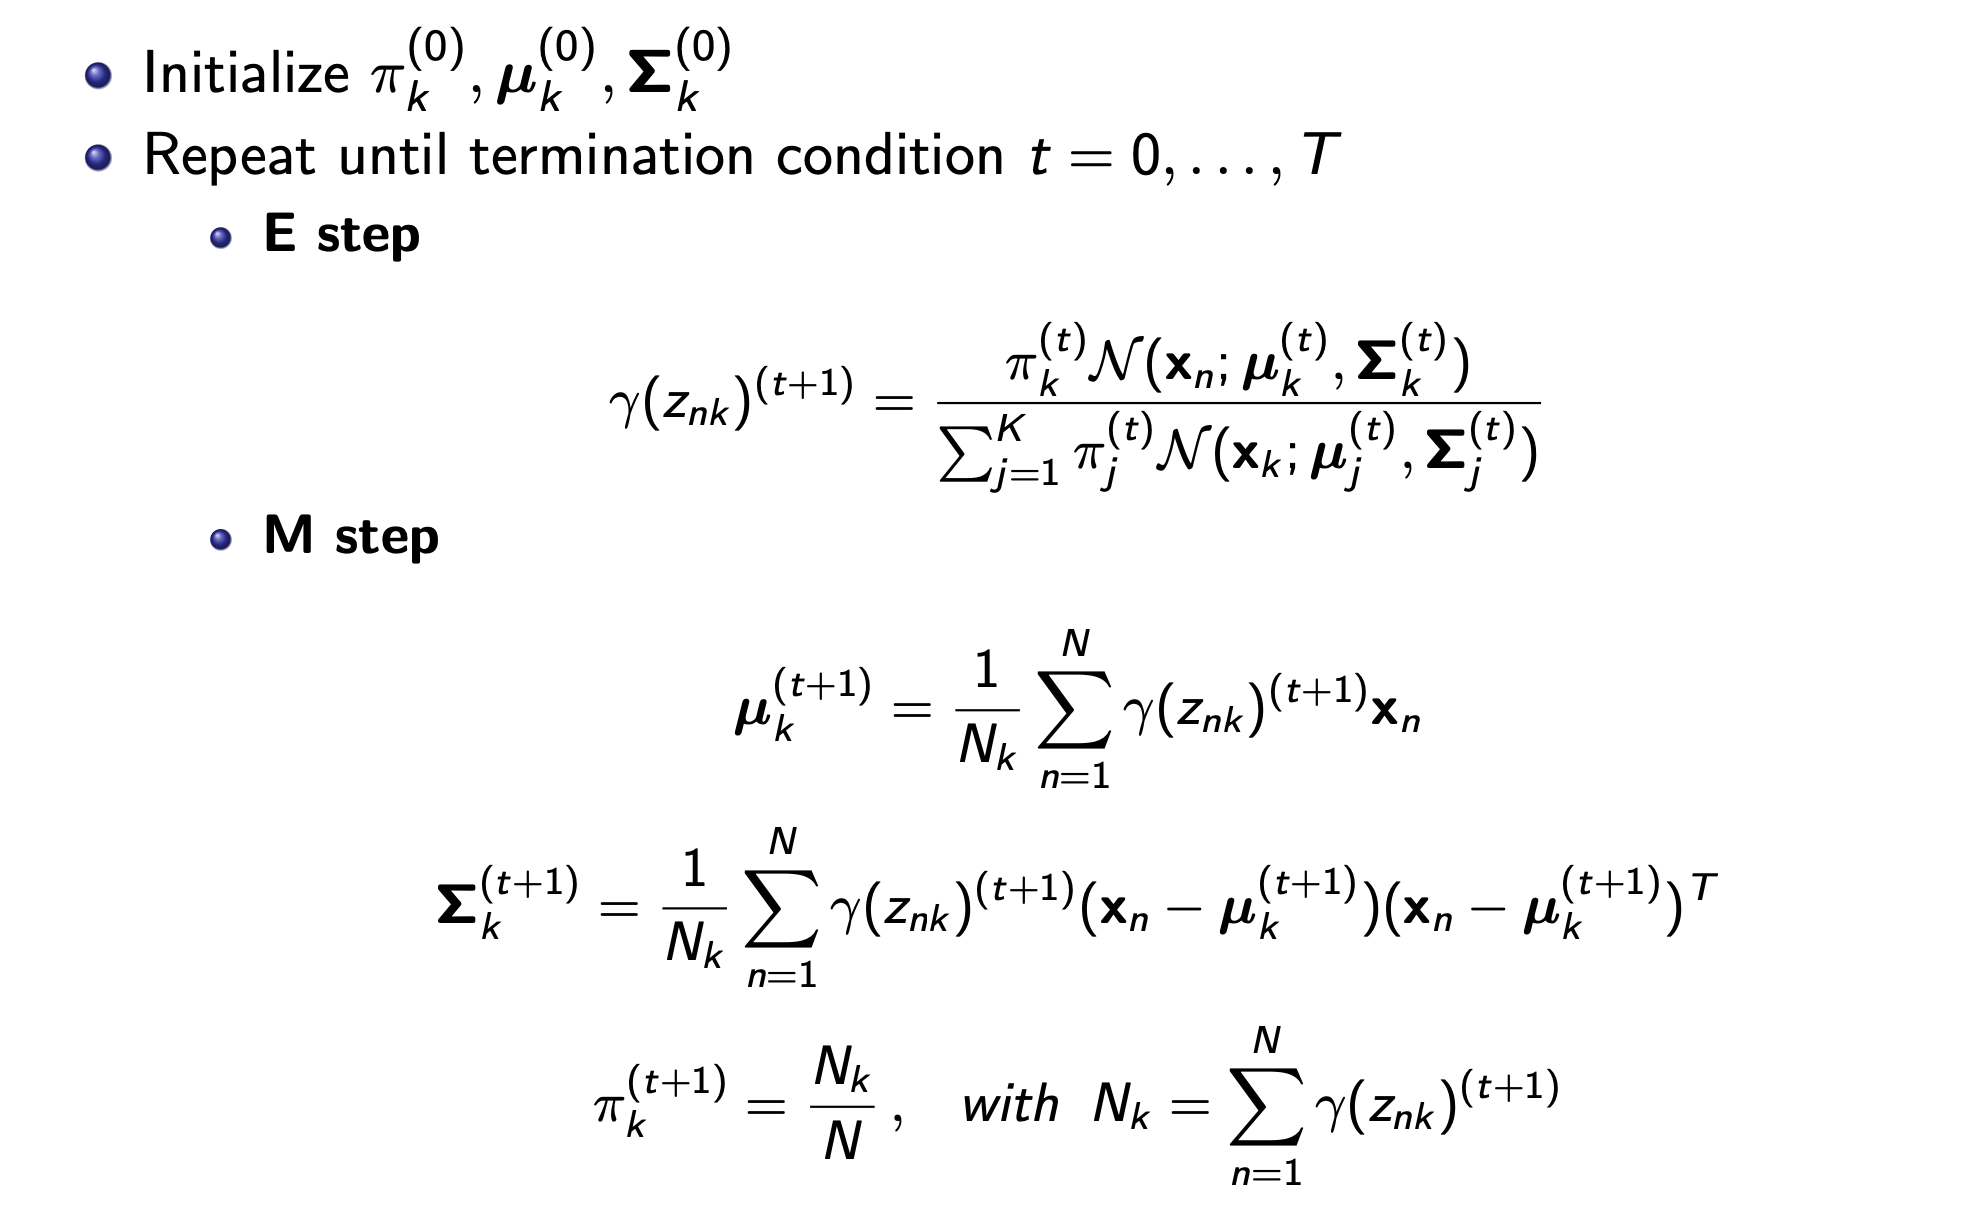
\includegraphics[scale=0.3]{gmm_em}
\end{figure}

\subsection{K-means}
In this one you first decide the number of clusters $K$. The you start the algorithm:
\begin{enumerate}
\item Partition the dataset into $K$ parts at random or use some kind of initialization algorithm
\item For each partition estimate the centroid $c_i=\frac{1}{N_k}\sum_k x_k$ 
\item For each sample $x$, compute two distances:
\begin{itemize}
\item Distance $d_i$ between $x$ and its current centroid $c_i$ 
\item Distance $d_{j}$ between the $x$ and the closest centroid $c_j$.
\end{itemize}
\item if $d_j<d_i$ assign $x$ to $d_j$
\item repeat until convergence
\end{enumerate}

\paragraph{Convergence}
Convergence is achieved if:
\begin{itemize}
\item The number of clusters $K$ is finite
\item $d_i$ decreases at each iteration 
\end{itemize}

\paragraph{Cons}
\begin{itemize}
\item K must be determined before hand
\item Sensitive to initial condition (local optimum) when a few data available.
\item Not robust to outliers. Very far data from the centroid may pull the centroid away from the real one.
\end{itemize}